\typeout{NT FILE chapter6.tex}
\chapter{Final model and evaluation}
\section{Final Model}

\section{Test Evaluation}

During the Training/ Validation/ Test split process 27 images were assigned to the test set, that is completely unseen data by the model. Using the best model frozen weights and architecture, inference is performed of the test dataset to assess model performance by comparing the predictions against the ground truth mask.

    \begin{figure}[hbt!]
        \centering
        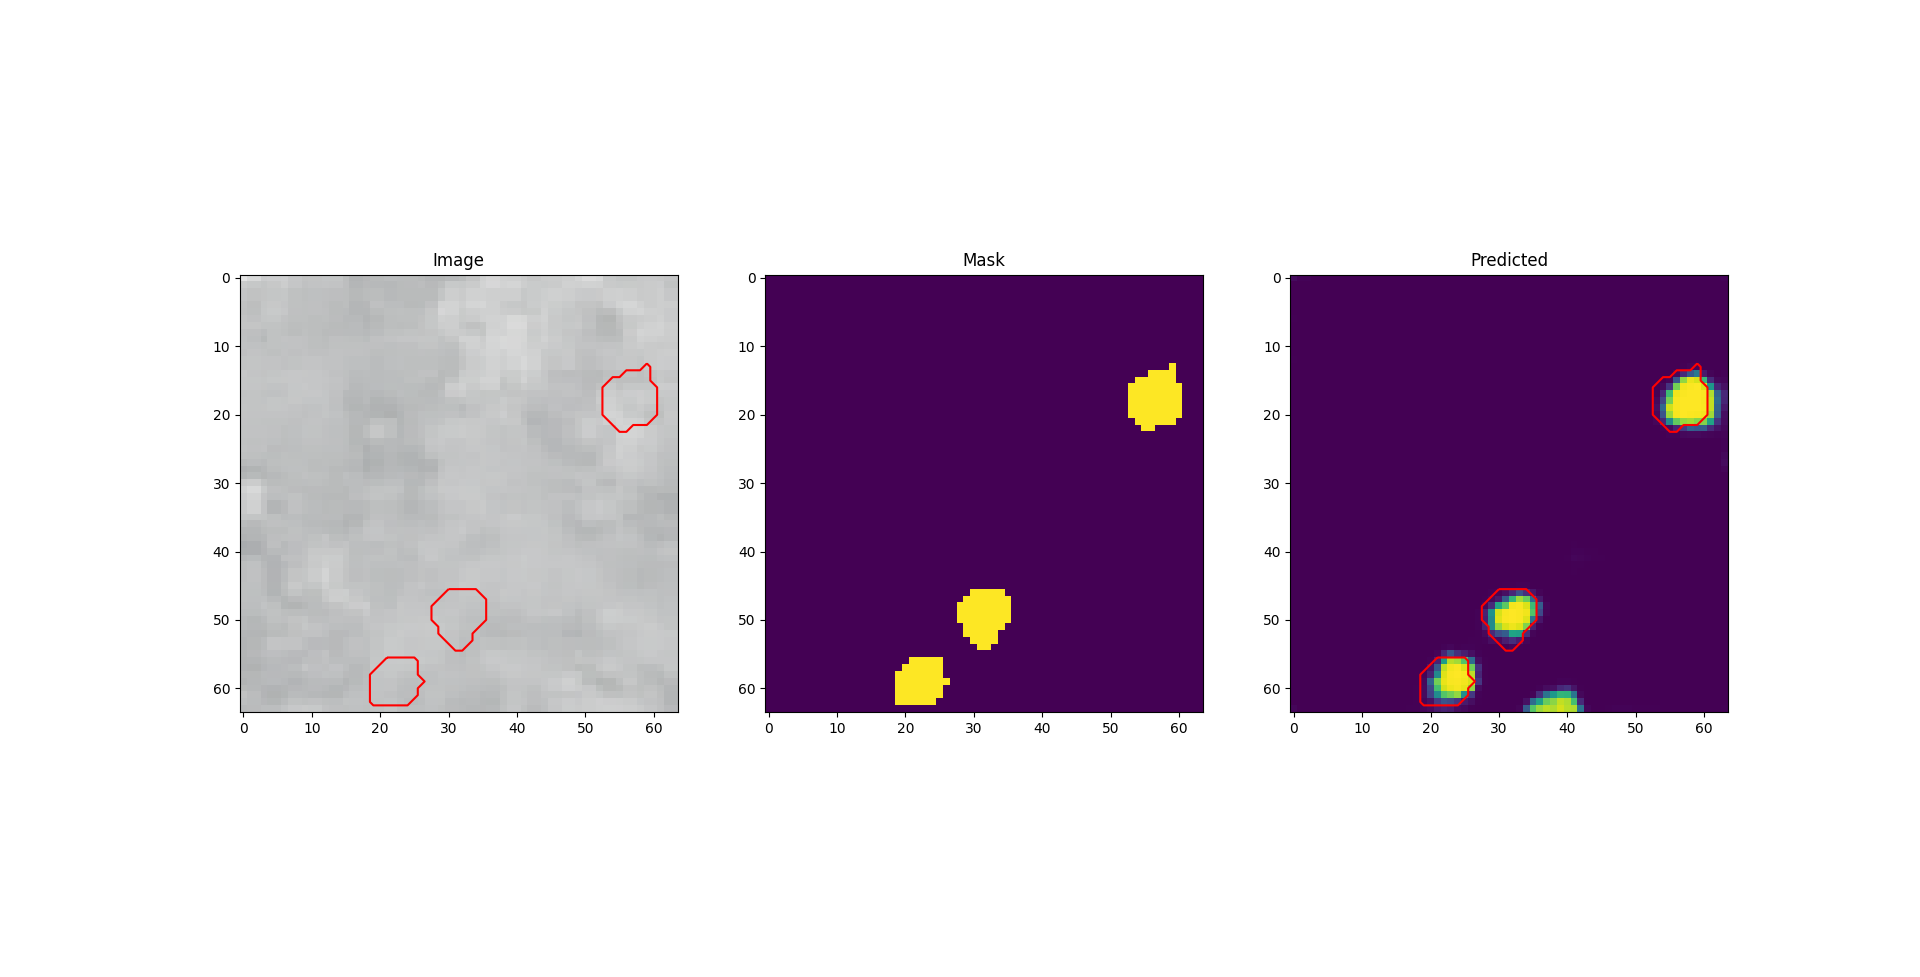
\includegraphics[width=1 \textwidth]{Figure_14_prediction multiple_fp.png}
        \caption{Test set predicted vs. ground truth example of True and False positives)}
        \label{fig_tp_fp}
    \end{figure}

